\documentclass[12pt,a4paper,]{article}
\usepackage{pdfpages}
\usepackage{lmodern}
\usepackage{amssymb,amsmath}
\usepackage{ifxetex,ifluatex}
\usepackage{fixltx2e} % provides \textsubscript
\ifnum 0\ifxetex 1\fi\ifluatex 1\fi=0 % if pdftex
  \usepackage[T1]{fontenc}
  \usepackage[utf8]{inputenc}
\else % if luatex or xelatex
  \ifxetex
    \usepackage{mathspec}
  \else
    \usepackage{fontspec}
  \fi
  \defaultfontfeatures{Ligatures=TeX,Scale=MatchLowercase}
\fi
% use upquote if available, for straight quotes in verbatim environments
\IfFileExists{upquote.sty}{\usepackage{upquote}}{}
% use microtype if available
\IfFileExists{microtype.sty}{%
\usepackage{microtype}
\UseMicrotypeSet[protrusion]{basicmath} % disable protrusion for tt fonts
}{}
\usepackage{hyperref}
\hypersetup{unicode=true,
            pdfborder={0 0 0},
            breaklinks=true}
\urlstyle{same}  % don't use monospace font for urls
\usepackage{graphicx,grffile}
\makeatletter
\def\maxwidth{\ifdim\Gin@nat@width>\linewidth\linewidth\else\Gin@nat@width\fi}
\def\maxheight{\ifdim\Gin@nat@height>\textheight\textheight\else\Gin@nat@height\fi}
\makeatother
% Scale images if necessary, so that they will not overflow the page
% margins by default, and it is still possible to overwrite the defaults
% using explicit options in \includegraphics[width, height, ...]{}
\setkeys{Gin}{width=\maxwidth,height=\maxheight,keepaspectratio}
% Make links footnotes instead of hotlinks:
\renewcommand{\href}[2]{#2\footnote{See \texttt{\url{#1}}}}
\setlength{\emergencystretch}{3em}  % prevent overfull lines
\providecommand{\tightlist}{%
  \setlength{\itemsep}{0pt}\setlength{\parskip}{0pt}}
\setcounter{secnumdepth}{5}
% Redefines (sub)paragraphs to behave more like sections
\ifx\paragraph\undefined\else
\let\oldparagraph\paragraph
\renewcommand{\paragraph}[1]{\oldparagraph{#1}\mbox{}}
\fi
\ifx\subparagraph\undefined\else
\let\oldsubparagraph\subparagraph
\renewcommand{\subparagraph}[1]{\oldsubparagraph{#1}\mbox{}}
\fi

\date{}


%
% Line Spread, Page Markings & Hyperlinked Documents
%
\linespread{1.3}
% Margin:
\usepackage[top=1.5in, bottom=1.5in, right=1in, left=1in]{geometry}

% To silence too small headheight warning
\setlength{\headheight}{15pt}

% Header & Footer:
\usepackage{fancyhdr}
\pagestyle{fancy}
\fancyhf{} % Clear all header and footer fields
\fancyhead[LO,RE]{Helpdesk Ticketing System\\{\vspace{-2pt}\scriptsize Semester 2}}
\fancyhead[LE,RO]{\leftmark\\{\vspace{-4pt}\scriptsize SWE40002 Software Engineering Project}}
\fancyfoot[LE,RO]{\thepage\ifodd\value{page}\else\hfill\fi}
\usepackage{float}

\begin{document}

{
\setcounter{tocdepth}{3}
\tableofcontents
}
\newpage
\section{Purpose}\label{purpose}

The purpose of the usability testing stage is to expose test candidates
to the HelpDesk Ticketing System, in order to collect data related to
their interactions with the system. All candidates will have a set of
tests to conduct, which involve utilising certain aspects of the
HelpDesk Ticketing System in order to achieve defined tasks.

The system that was being used prior to the implementation of the
HelpDesk Ticketing System is based on the same principle, where a queue
is implemented, in which students place their name and the task that
they need assistance with. The model revolved around students entering
their name into a list defined within a text editor. The image in Figure
1 offers a representation of how the previous system worked.

\begin{figure}[htbp]
\centering
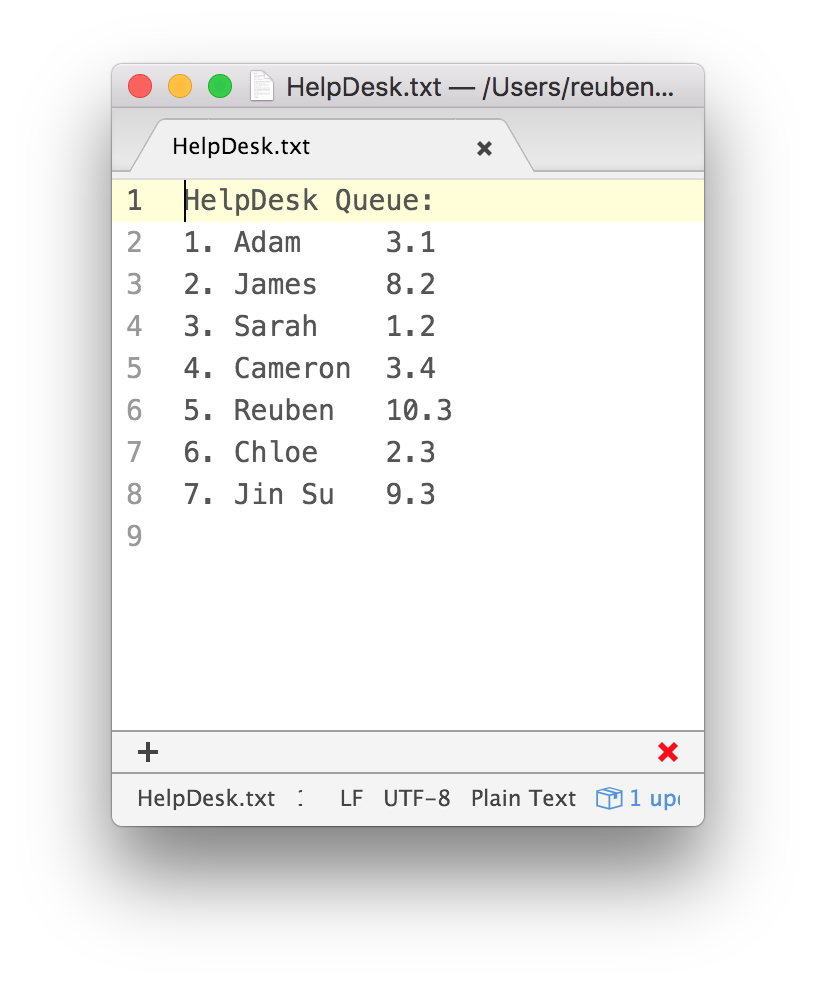
\includegraphics{1.png}
\caption{Previous Helpdesk System}
\end{figure}

The idea behind the text editor based HelpDesk queue is the same as the
idea that pushed the development of the HelpDesk Ticketing System; have
a way to visualise the help that is required for students, and serve
them in a first in, first out fashion. Once they have had their problem
resolved, remove them from the queue and move onto the next student. One
of the major limitations with the previous model include relates to the
fact that no data or metrics were being recorded in regards to the
assistance being provided at the HelpDesk, which directly influences the
way that help provided can be catered and changed to suit the most
common issues students face within their units of study.

It is important to understand that no surveys were conducted in regards
to what HelpDesk users, both students and staff, thought of the
implementation prior to developing the HelpDesk Ticketing System. That
being said though, some generalized data was collected through surveying
test participants, which directly correlates to how they would ideally
invisage their interactions with the HelpDesk. The collected results are
highlighted within the data collection appendix, under the heading
\emph{HelpDesk Attendance}.

During the testing phase, a high fidelity prototype was provided to test
participants to sample, and by using such a prototype, all test
participants were able to complete critical tasks, such as created a
support ticket etc.

After the testing phase, all participants were required to complete
relevant feedback surveys in order to be able to collect data related to
their interactions with the HelpDesk Ticketing prototype. The surveys,
and related data, can be found within the data collection appendix.

\section{Scope}\label{scope}

What was tested:

\subsection{Font Sizes}\label{font-sizes}

At various positions in the room, how well can subjects read various
font sizes for text which is displayed on a projector. Refer to Figure
2.

\begin{figure}[htbp]
\centering
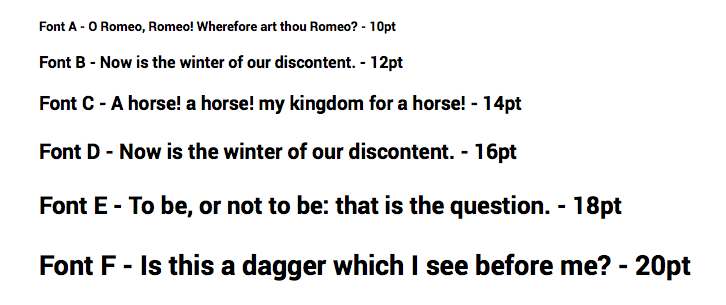
\includegraphics{2.png}
\caption{Font size test}
\end{figure}

\subsection{Basic Scenarios}\label{basic-scenarios}

Ask test subjects to perform various use scenarios to see if and how
long it takes for someone to complete a particular task. Refer to the
task descriptions in the appendix.

\subsection{Interpretation of
dashboard}\label{interpretation-of-dashboard}

How well were subjects able to gather information from the dashboard.

\subsection{Mobile site navigation}\label{mobile-site-navigation}

How well were subjects able to navigate the mobile version of the
system.

We are not testing:

\subsection{User assumption}\label{user-assumption}

We assumed all users are familiar with basic PC input like mouse and
keyboard, this is due to the nature of the end users of the system.

We assumed all users are familiar with basic web page navigation, menu
styles and standards etc.

\section{Test Strategy}\label{test-strategy}

The strategy chosen for usability testing will be in two parts. For both
parts, the usability evaluator will be with the participant.

\subsection{Surveys}\label{surveys}

Firstly the participants will fill out a survey, what they think about
how the current helpdesk works and their ideal expectations. In
addition, some demographic details will also be collected.

\subsection{Live Testing with
Participants}\label{live-testing-with-participants}

Secondly the participants will use a prototype of the helpdesk ticketing
system and attempt to perform a number of defined tasks. The evaluator
may help the participant if they get stuck on a task. During this time,
the evaluator will make notes about any difficulties had, or comments
made, by the participant. These details, and the surveys results, become
the combined results of the evaluation.

\subsection{Post-Test Evaluation}\label{post-test-evaluation}

After the participant has completed the tasks, they will be asked to
evaluate the prototype using the standard System Usability Scale
questions. This will provide useful data on what could be improved with
the prototype.

\section{Environment}\label{environment}

The test was held in ATC621, a similar environment to the actual
helpdesk where the end system will be deployed. The reason it was held
in this room is that we were not able to disturb the helpdesk. The test
made use of:

\begin{itemize}
\tightlist
\item
  \textbf{A projector}: An Epson projector, same as which will be used
  in the HelpDesk.
\item
  \textbf{PC}: Macbook Air with trackpad used to display the prototype.
\item
  \textbf{Web Browser}: Google Chrome, the same as which will be used in
  the Helpdesk.
\item
  \textbf{Mobile chrome view}: Used to simulate phone browser built into
  Google Chrome.
\item
  \textbf{Keyboard/Mouse}: Same as which will be used in Helpdesk.
\end{itemize}

\section{Discussion of Results}\label{discussion-of-results}

\subsection{Participant Demographics}\label{participant-demographics}

In terms of demographics, there was a limitation in that most
participants were male and young. Although this does generally fit the
demographics of people enrolled in programming units. The tutors that
participated were all very experienced (4 or more semesters of
tutoring).

\subsection{Expectations of the Help
Desk}\label{expectations-of-the-help-desk}

Students were unanimous in being willing to wait 6 minutes or more for
getting help in the help desk, which is more than what they report
currently waiting. Student were generally not from using the helpdesk if
the helpdesk was busy. The most helpful information that students wanted
to know in advance before going to the help desk were: how many tutors
are on duty, the units taught by the tutors and a simple description of
how busy it is.

Tutors reported being able to support 4-5 students without being
overburdened and they generally concurred with students in term of
appropriate student wait time. The most helpful information tutors would
like before helping a student were: the student's name and the unit and
task they need help with.

The information desired by both students and tutors was generally in
line with the interface of the prototype that the participants then went
on to use.

\subsection{Things Participant Liked about the
Prototype}\label{things-participant-liked-about-the-prototype}

Participants were found to like the following attributes:

\begin{itemize}
\tightlist
\item
  Doing the major tasks like creating tickets, clocking on/off and
  viewing the queue did not present much difficulty to the participants.
\item
  For students, being able to see which tutors are clocked on and what
  units they each was very useful to them.
\item
  Tutors liked the clocking on/off feature
\item
  Participants liked the mobile support of the dashboard.
\end{itemize}

In terms of the System Usability Scale evaluation results, the
participants gave overwhelmingly positive feedback, with some
exceptions. See the appendix for the full listing of results from the
evaluations.

\subsection{Things Participant Thought Could be Better about the
Prototype}\label{things-participant-thought-could-be-better-about-the-prototype}

Participants were found not to like the following attributes

\begin{itemize}
\tightlist
\item
  Complex graph - some participants thought the graph showed too much
  information, the descriptive text of the axis was hard to read and/or
  it was not presented in a way that could convey the activity level of
  the help desk.
\item
  Clock In Time - some participants found the decimal measure of hours
  (i.e.~0.75 meaning 45 minutes) not as intuitive as how fractions of
  hours are normally displayed.
\end{itemize}

\appendix

\newpage

\section{General Instructions}

See attached document

% \clearpage
% \ifodd\value{page}\hbox{}\newpage\fi

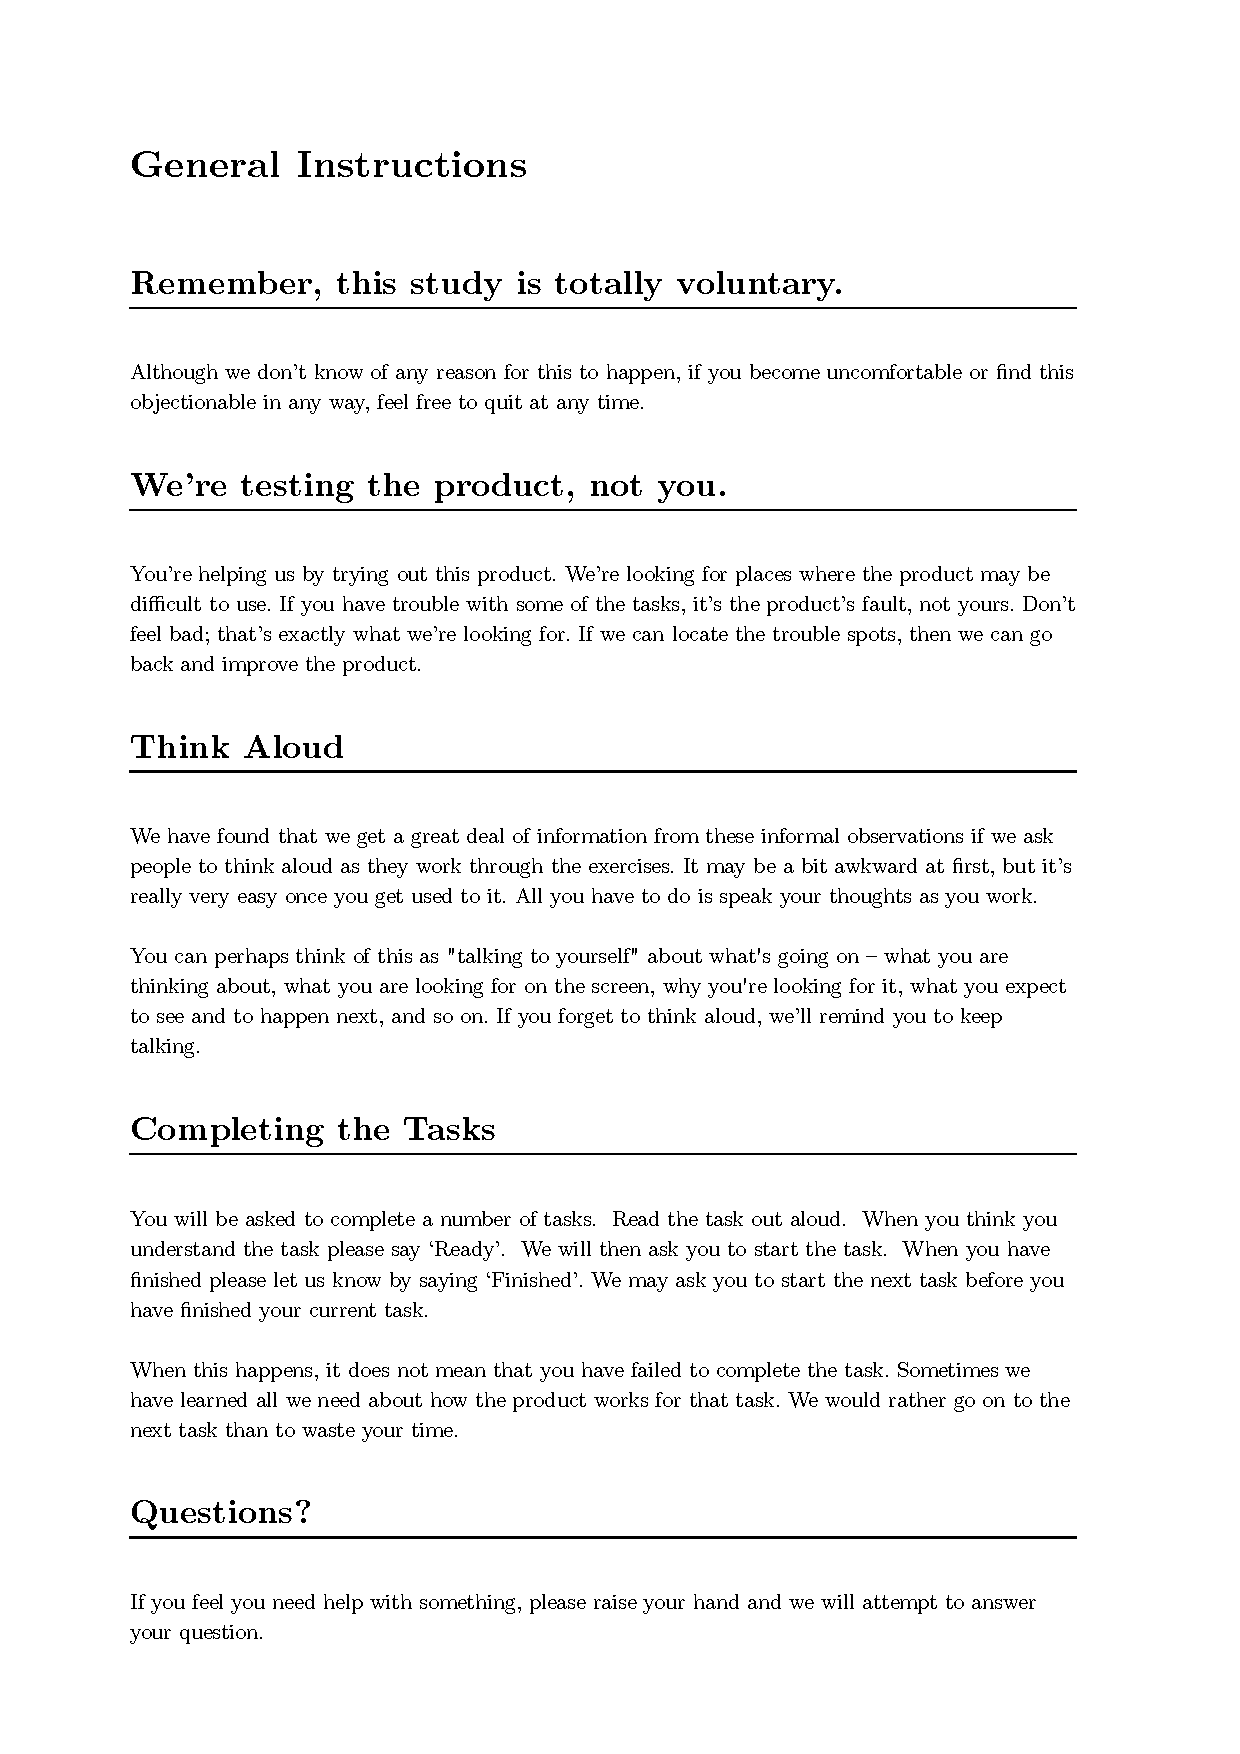
\includepdf[pages={-}]{1.pdf}

\section{Pre-Evaluation Survey}

See attached document

% \clearpage
% \ifodd\value{page}\hbox{}\newpage\fi

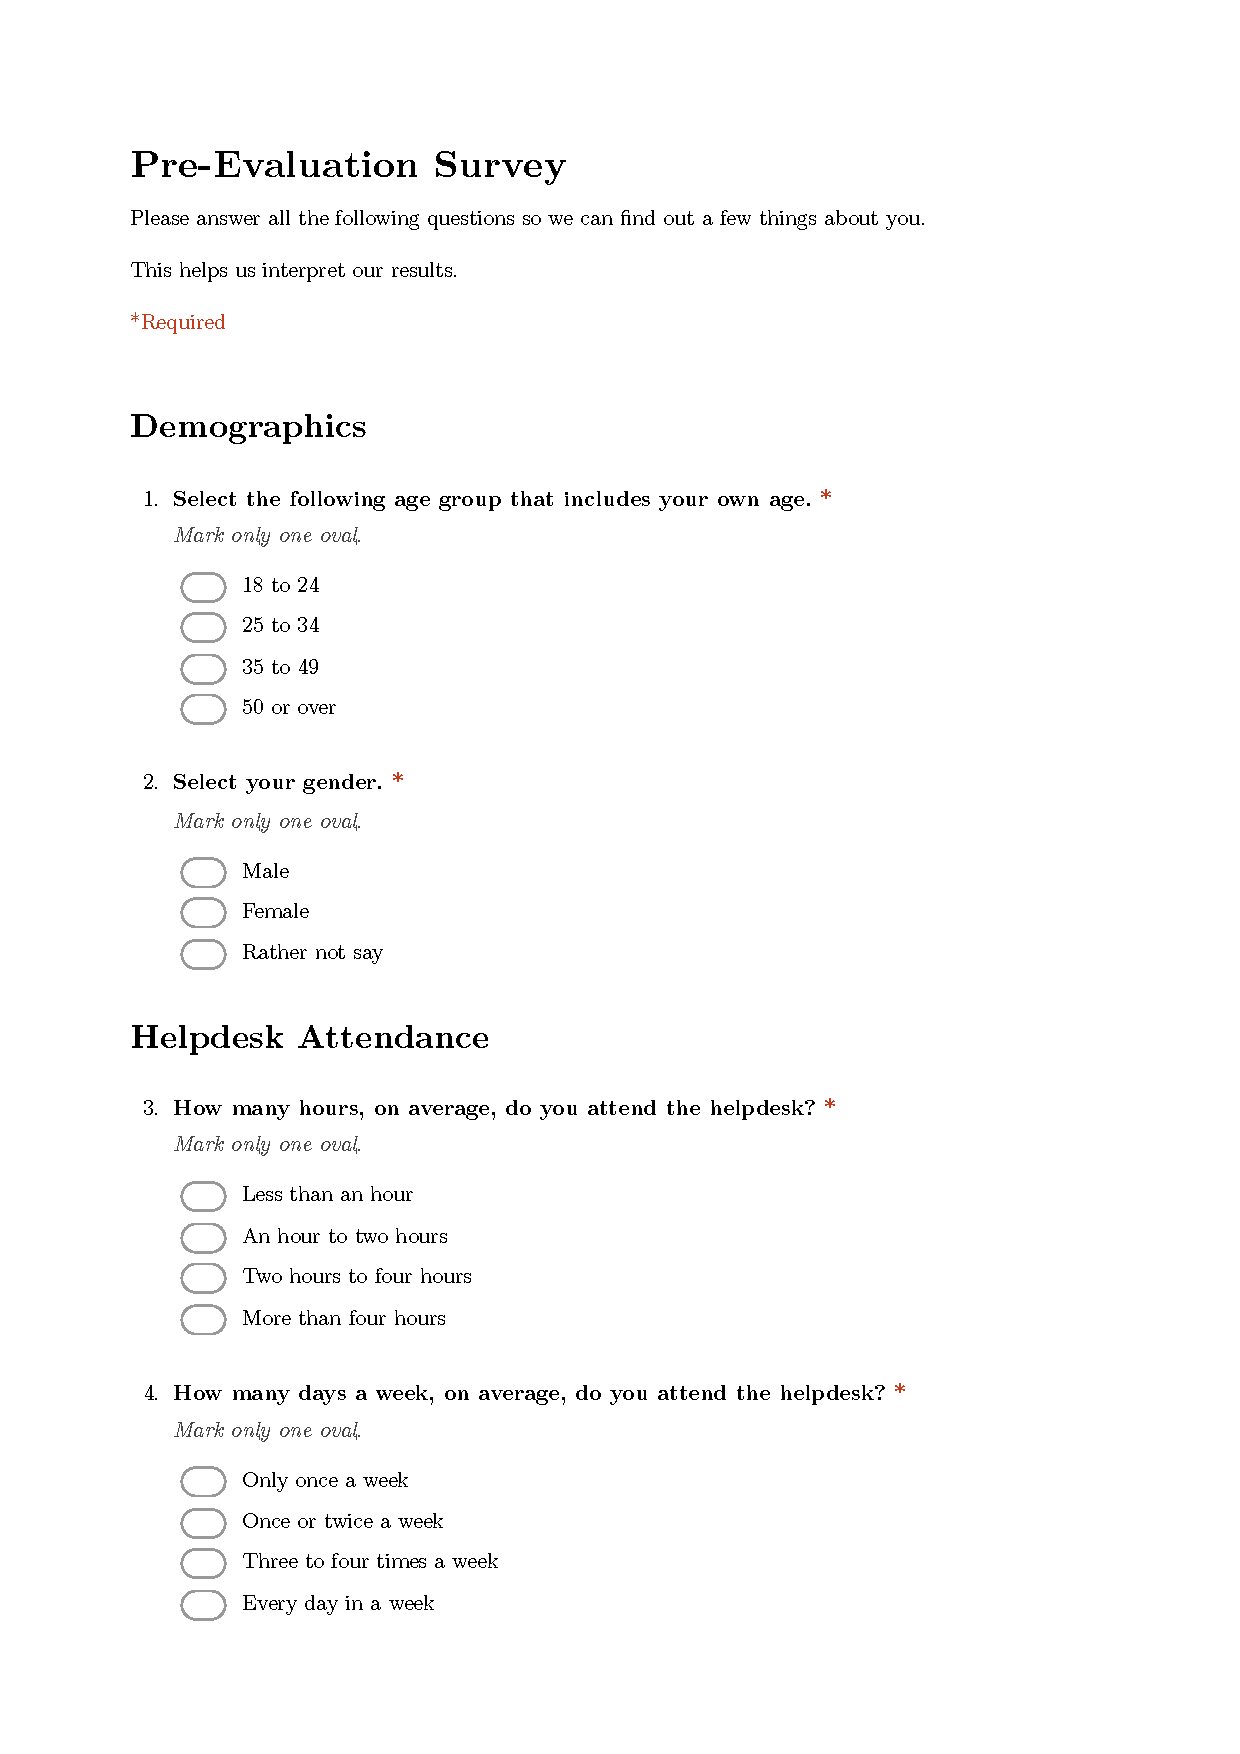
\includepdf[pages={-}]{2.pdf}

\section{Raw Results}

See attached document

% \clearpage
% \ifodd\value{page}\hbox{}\newpage\fi

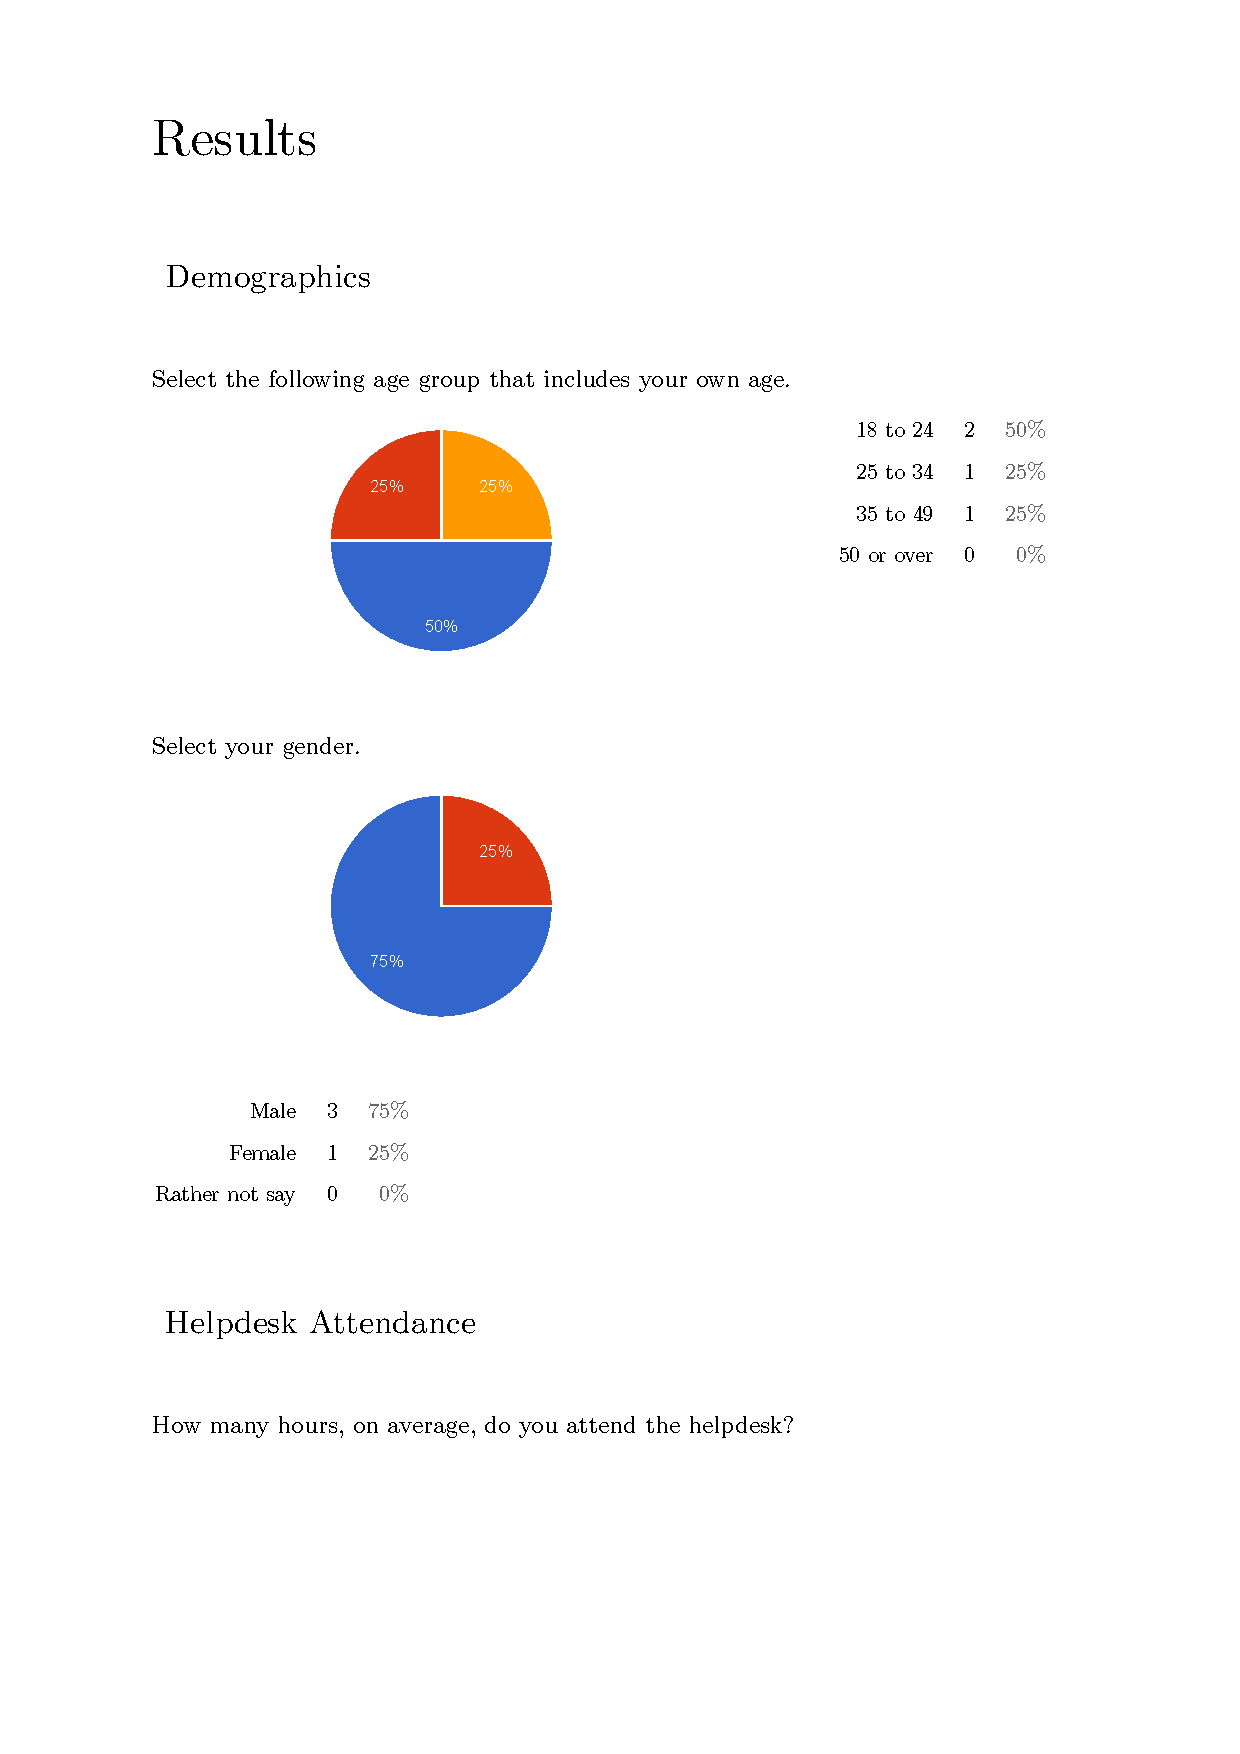
\includepdf[pages={-}]{3.pdf}

\section{User Evaluation Consent Forms}

See attached document

% \clearpage
% \ifodd\value{page}\hbox{}\newpage\fi

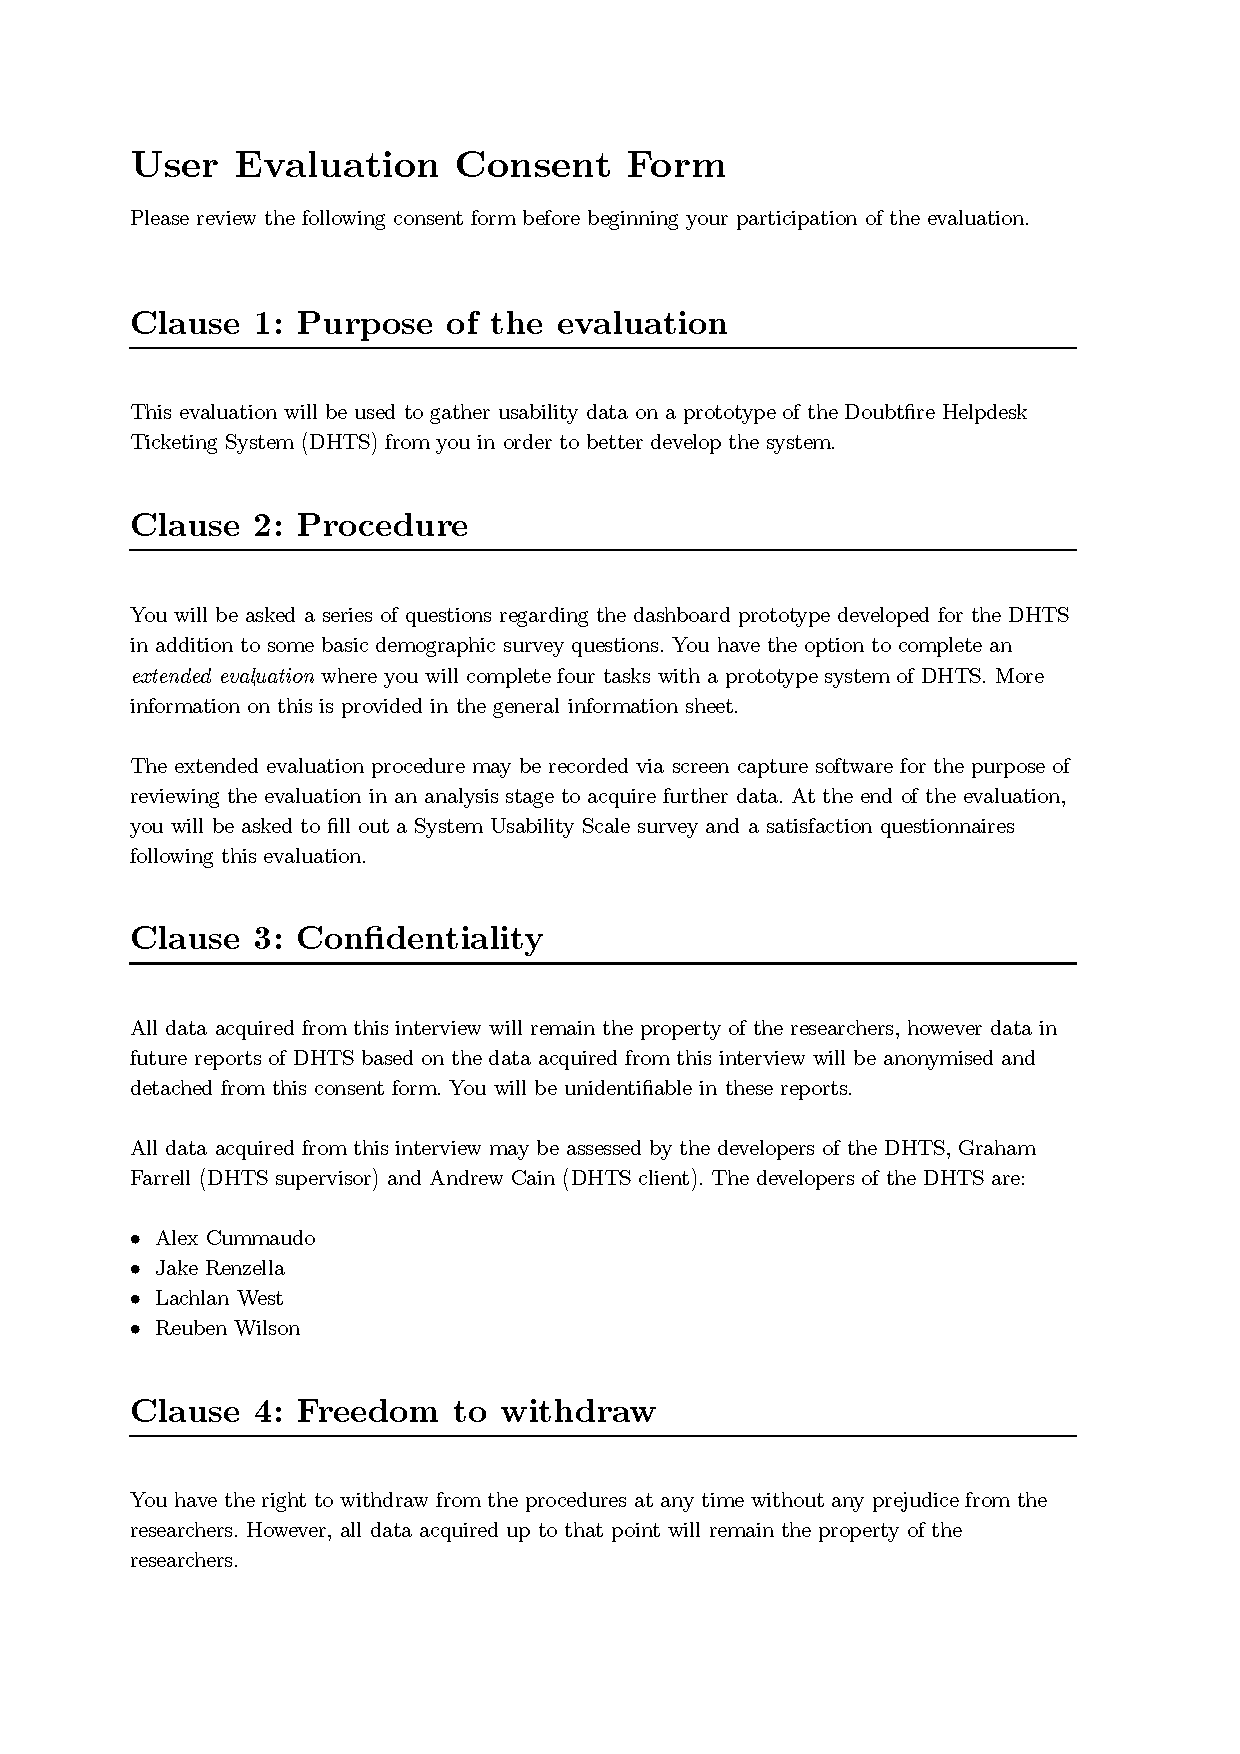
\includepdf[pages={-}]{4.pdf}

\end{document}
